\documentclass[10pt]{article}
\usepackage[margin=1in]{geometry}
\usepackage[T1]{fontenc}
\usepackage{mathptmx}
\usepackage{amsmath,amssymb,amsthm}
\usepackage{fancyhdr}
\usepackage{graphicx}
\usepackage{listings}
\usepackage{float}
\usepackage{booktabs}
\usepackage[numbers,sort&compress]{natbib}
\usepackage[hidelinks]{hyperref}
\usepackage[expansion=false]{microtype}
\usepackage{enumitem}
\usepackage{titlesec}

\titlespacing*{\section}{0pt}{7pt plus 2pt}{3pt}
\titlespacing*{\subsection}{0pt}{5pt plus 2pt}{2pt}
\titleformat*{\section}{\large\bfseries}
\titleformat*{\subsection}{\normalsize\bfseries}
\setlength{\parskip}{2pt}
\setlength{\abovedisplayskip}{4pt}\setlength{\belowdisplayskip}{4pt}
\setlength{\textfloatsep}{8pt plus 2pt}
\setlength{\floatsep}{6pt}
\setlength{\abovecaptionskip}{3pt}
\newtheorem{prop}{Property}
\newcommand{\xc}{x_{\mathrm{crit}}}

\pagestyle{fancy}
\fancyhf{}
\lhead{\small CS/INFO 6850 Exploratory Paper}
\rhead{\small Cascading Failures in Supply Networks}
\cfoot{\small\thepage}
\renewcommand{\headrulewidth}{0.3pt}

\title{\vspace{-2.2em}\Large\bfseries Redundancy, Geography, and the Supply-Network Precipice:\\ \large k-of-n Multisourcing under Correlated Regional Shocks}
\author{Arjun Saini \and Aryavardhan Singh\\ \small CS/INFO 6850: The Structure of Information Networks, Cornell University, Fall 2026}
\date{\small November 2, 2026}

\begin{document}
\maketitle
\thispagestyle{fancy}
\vspace{-1.6em}

\begin{abstract}
\noindent
When does the failure of a few firms or regions cascade into a collapse of production? Elliott, Golub, and Leduc \cite{egl2022} (EGL) predict a discontinuous ``precipice'' in output, while Carvalho, Nirei, Saito, and Tahbaz-Salehi \cite{cnst2021} (CNST) find that the 2011 Japanese earthquake propagated smoothly, decaying with network distance. Neither paper captures how redundant sourcing interacts with geographically correlated shocks. We extend EGL's model so that a firm needs $k$ of its $n$ suppliers per input, with suppliers grouped into regions that fail together. We prove that a redundancy requirement creates a precipice even when firms need only one input and that perfectly spread suppliers turn a regional shock into exactly EGL's economy-wide shock, and we find that co-locating suppliers lowers the collapse threshold in every case tested. Simulations on finite networks match the theory (mean absolute error 0.0025), confirm all-or-nothing outcomes at the threshold, and show that a shock to one region holding 0.5\% of firms but 11\% of supply relationships can collapse a network whose firms need two working suppliers.
\end{abstract}

\section{Introduction}
In a supply network a cascade has a direct economic cost: a firm missing one essential input cannot produce, and its customers then face the same problem. The question joins two course units, Cascading Behavior (threshold rules on neighbors) and Random Graphs (branching processes, phase transitions, the giant component). We ask how \emph{redundancy} (needing several working suppliers) and \emph{geography} (suppliers that fail together) move the point at which a supply network collapses.

We anchored the search on EGL \cite{egl2022}, followed papers citing it from 2021 to 2026, and ran keyword sweeps on production-network fragility, percolation with redundancy, and correlated shocks. We scored candidates on relevance to the redundancy and correlated-shock question, impact, recency, and whether they support both analysis and simulation. We chose CNST \cite{cnst2021} as the companion because it is a widely cited, top-journal empirical study and because its shock is regional, which is exactly the ingredient EGL leave out. Neither paper is linked from the course page. Sections 2 and 3 analyze the two papers, Section 4 contrasts them, Section 5 develops our model, and Section 6 tests it on simulated networks.

\section{Paper 1: Elliott, Golub, and Leduc (2022), ``Supply Network Formation and Fragility''}
\paragraph{Technical content.} A continuum of firms is arranged in deep random supply trees. A firm at depth $d>0$ needs $m$ distinct essential inputs and, for each, has $n$ potential suppliers at depth $d-1$. Each sourcing relationship is operational independently with probability $x$ (the \emph{relationship strength}), and a firm is functional if, for every input, at least one operational supplier is itself functional. If $r$ is the probability that a depth-$(d-1)$ firm works, a supplier is usable with probability $xr$, so
\begin{equation}
r_d = R_x(r_{d-1}), \qquad R_x(r) = \bigl(1-(1-xr)^n\bigr)^m .
\label{eq:egl}
\end{equation}
Deep networks converge to the largest fixed point of $R_x$. For $m\ge 2$, $R_x$ is convex then concave, so as $x$ falls the largest crossing with the diagonal reaches a tangency and disappears. Reliability (the probability a firm works) therefore jumps from a positive value to zero as $x$ falls below a critical strength $\xc$, with an infinite slope just above it (their Proposition 1). For example, with $m=2$ and $n=4$ we compute $\xc=0.518$, where reliability drops from $0.64$ to $0$. With $m=1$ the map is concave and the transition is continuous; since $R_x'(0)=nx$, it occurs at $x=1/n$. EGL then make $x$ endogenous: each firm pays to raise its own relationship strength above a baseline $\underline{x}$, at a cost scaled by $1/\kappa$, but does not account for how its reliability helps its customers and their customers. For $m\ge3$, on a whole interval of the cost parameter $\kappa$ the equilibrium sits within $\varepsilon$ of $\xc$ (their Theorem 1), because near equilibrium each firm's investment substitutes for its suppliers'. On that interval an arbitrarily small drop in $\underline{x}$ sends reliability to roughly zero (Proposition 3), while a social planner never chooses $x$ near $\xc$ (Proposition 2), so these equilibria are both fragile and very inefficient.

\paragraph{Course connections.} The functionality rule is a deterministic threshold rule, an AND across inputs of an OR across suppliers, so it is the mirror image of the adoption cascades of Granovetter \cite{granovetter1978} and Easley and Kleinberg \cite[\S19.7]{ek2010}: a node deactivates when its support falls below threshold. With $m\ge2$ the rule is a complex contagion \cite{centola2007}. The case $m=1$ is survival of a Galton--Watson tree with mean offspring $nx$, the same mechanism as the Erd\H{o}s--R\'enyi giant component (which EGL also note), while $m\ge 2$ produces a discontinuous (first-order) transition like $k$-core percolation \cite{dorogovtsev2006} or interdependent-network cascades \cite{buldyrev2010}. In the ``economic issues'' view of cascades \cite{kleinberg2007}, the novelty is that the threshold is set by strategic play rather than given.

\paragraph{Weaknesses and directions.} The most important limitation for us is that link failures are independent, and the only aggregate shock is a uniform drop in $x$. Real shocks (earthquakes, port closures) are geographically correlated, so co-located suppliers fail together and multisourcing protects less than the model implies. The ``at least one supplier'' rule also ignores capacity: one surviving supplier rarely replaces four. Additionally, the depth-ordered tree has no hubs or cycles, failures pass only from suppliers to their customers (a simplification EGL acknowledge), the main theorem requires $m\ge 3$ (they support $m=2$ only numerically), and neither $x$ nor $\xc$ is observable, which makes the precipice hard to falsify. Sections 5 and 6 address the first two issues with a $k$-of-$n$ rule and regional shocks.

\section{Paper 2: Carvalho, Nirei, Saito, and Tahbaz-Salehi (2021), ``Supply Chain Disruptions''}
\paragraph{Technical content.} The March 2011 earthquake and tsunami hit four prefectures producing 4.6\% of Japan's output. Their GDP growth fell 2.2 percentage points (pp), which directly accounts for only about 0.1pp of national growth, yet national growth fell roughly 0.43pp. Using a Tokyo Shoko Research panel of 750{,}237 firms with binary supplier--customer links (about 5 suppliers and 5.6 customers per firm, with Pareto degree tails of shape about 1.25--1.3), CNST assign each firm an upstream and downstream network distance to the disaster area and estimate a difference-in-differences model with firm and prefecture$\times$industry$\times$year fixed effects. In the following year, sales growth fell by 3.8pp for firms whose suppliers were in the disaster area (``downstream'' distance 1) and by 3.1pp for firms whose customers were (``upstream'' distance 1), with effects decaying over further hops and no pre-trends. The results survive restricting to single-plant firms, splitting Japan by its two electricity grids, and a placebo network that randomly rewires links while keeping each firm's number of customers. A nested-CES general equilibrium model, with the disaster as a capital shock, then uses these estimates to identify two elasticities: primary and intermediate inputs are complements ($\sigma\approx0.60$) and different intermediate inputs are mild substitutes ($\xi\approx1.18$). The calibrated model attributes a 0.47pp drop in real GDP growth to the disaster. Cutting all input--output links between firms inside and outside the disaster area would have limited it to 0.21pp, so propagation to the rest of the country more than doubled the loss.

\paragraph{Course connections.} This is one of the cleanest causal measurements of contagion on a real network, and the pattern (decay per hop, effects in both directions) resembles an attenuating simple contagion rather than a threshold cascade. Their Leontief inverse $L=(I-\mu A)^{-1}=\sum_{r\ge0}(\mu A)^r$, with $A$ the firm input--output matrix and $\mu=0.5$ the intermediate-input share, is a damped sum over all walks in the network. This is the structure of Katz centrality and PageRank \cite[\S14.6]{ek2010}, and CNST compute it the same way, by truncating the series. The rewired placebo is a configuration-model-style null.

\paragraph{Weaknesses and directions.} The structural model is linearized around Cobb--Douglas, so thresholds and discontinuities are ruled out by construction and the framework cannot detect an EGL-style precipice. Exposure is measured as minimum network distance, which treats a firm with 1 of 10 suppliers in the disaster area the same as one with 10 of 10, discarding exactly the redundancy dimension. The link weights $a_{ij}$ are imputed from industry-level input--output tables, since only binary links are observed, and the panel requires sales in all three years, so firms that exited (the outcome most diagnostic of collapse) drop out. Section 7 proposes tests that address these gaps.

\begin{figure}[!t]
\centering
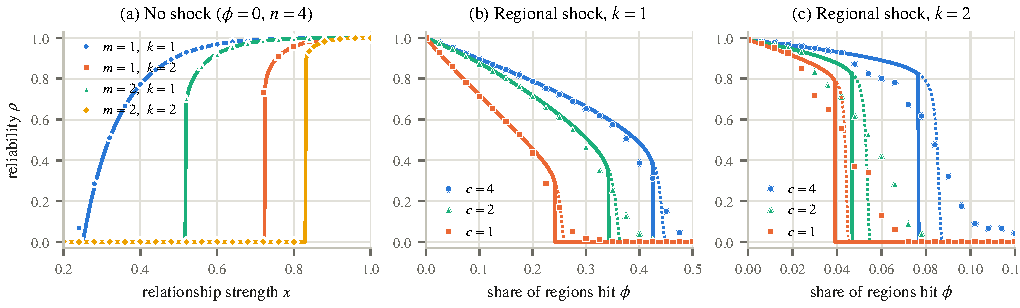
\includegraphics[width=\linewidth]{figures/fig_validation.pdf}
\caption{Simulation (markers, mean over replications) against theory (solid: infinite depth; dotted: depth 20). (a) Reliability against relationship strength with no shock: $k=2$ creates a jump even with one input. (b, c) Reliability against the share of regions hit for $m=2$, $n=4$, $x=0.9$: co-located suppliers ($c=1$) collapse first, and $k=2$ shrinks the tolerable shock more than fivefold.}
\label{fig:validation}
\end{figure}

\section{Synthesis: Knife-Edge Collapse versus Smooth Propagation}
EGL predict all-or-nothing failure with equilibrium forces pushing the economy toward the edge, while CNST find smooth propagation that decays with distance yet still roughly doubles the national loss. They are less contradictory than they look. CNST's linearized model cannot generate a jump, their outcome is average sales growth among surviving firms, and EGL themselves show that networks above the critical range are robust to small shocks. So CNST's evidence is consistent with a Japanese network that was \emph{not} critical in 2011. However, neither paper covers how redundancy interacts with correlated shocks: EGL's protection is multisourcing but their shocks are independent, while CNST's shock is spatially correlated but their model has no redundant suppliers. Our model sits in this gap and asks when spreading suppliers across regions really diversifies risk.

\section{Proposed Model: k-of-n Multisourcing with Regional Shocks}
\paragraph{Setup.} We keep EGL's deep random trees with $m$ inputs, $n$ potential suppliers per input, and strength $x$, and make two changes. First, an input is sourced only if at least $k$ of its $n$ suppliers are both functional and linked by an operational relationship, which models capacity limits (each supplier covers only part of the need) or dual-sourcing mandates; $k=1$ recovers EGL. Second, there are many regions, each hit independently with probability $\phi$ (so $\phi$ is the expected share of regions hit), and every firm in a hit region fails. A firm's $n$ suppliers for each input are split into $c$ clusters of $b=n/c$, all suppliers in a cluster share one region, and different clusters sit in independently drawn regions. With $n=4$, $c=4$ means fully spread suppliers, $c=2$ two co-located pairs, and $c=1$ all four in one region. Let $S_k(N,p)=\Pr[\mathrm{Bin}(N,p)\ge k]$, and let $r$ be the probability that a deep firm works given that its own region survives. An input has $C\sim\mathrm{Bin}(c,1-\phi)$ surviving clusters, hence $Cb$ surviving suppliers, each usable independently with probability $xr$. A firm needs all $m$ inputs, so
\begin{equation}
r = F(r) := \Bigl[\,\sum_{C=0}^{c}\tbinom{c}{C}(1-\phi)^C\phi^{c-C}\,S_k(Cb,\,xr)\Bigr]^m, \qquad \rho=(1-\phi)\,r^*,
\label{eq:model}
\end{equation}
where $r^*$ is the largest fixed point and $\rho$, the aggregate reliability, also requires the firm's own region to survive. We define $\xc(k,n,m)$ as the smallest $x$ with a positive fixed point when $\phi=0$, and the collapse threshold $\phi^*$ as the largest $\phi$ with $r^*>0$.

\begin{prop}[Redundancy creates a precipice]
If $k\ge2$, the transition is discontinuous even with simple production ($m=1$).
\end{prop}
\noindent Take $\phi=0$. Near $r=0$, $S_k(n,xr)\approx\binom{n}{k}(xr)^k$, so $F'(0)=0$ and $F$ lies below the diagonal near the origin. Reliability therefore cannot grow continuously out of zero: as $x$ rises, a positive fixed point first appears where $F$ touches the diagonal at a strictly positive $r$, which is a jump. With $k=1$, $F'(0)=nx$, so a positive fixed point grows continuously from zero once $nx>1$. EGL trace the precipice to complexity ($m\ge2$), but this shows the real cause is needing several things to work at once, whether different inputs or several suppliers of one input. For $m=1$, $n=4$, $k=2$ we compute $\xc=0.725$ with a jump to $r^*=0.75$, as shown in Figure~\ref{fig:validation}(a).

\begin{prop}[Spread suppliers turn regional shocks into systemic ones]
If $c=n$, then $F(r)=[S_k(n,(1-\phi)xr)]^m$, so the regional shock is exactly a drop in strength from $x$ to $(1-\phi)x$, and $\phi^*=1-\xc(k,n,m)/x$.
\end{prop}
\noindent This follows from binomial thinning: a supplier survives its region with probability $1-\phi$ and is usable with probability $xr$, independently across suppliers. So full geographic diversification turns a lumpy regional shock into precisely EGL's systemic shock, and a network in a critical equilibrium ($x\approx\xc$) collapses under an arbitrarily small regional shock even with perfectly spread suppliers.

\begin{prop}[Co-location defeats multisourcing]
If $c=1$, then $F(r)=(1-\phi)^m[S_k(n,xr)]^m$. With probability $\phi$ the one region holding all of an input's suppliers is hit and the input fails no matter how large $n$ is, so adding suppliers in the same region offers no protection against the shock.
\end{prop}
\noindent \textbf{Conjecture (geography is monotone).} In every case we computed, $\phi^*$ increases with $c$. A proof needs a stochastic-ordering argument on the surviving-supplier count, which is not immediate because $S_k$ is neither convex nor concave in that count.

\paragraph{Worked example.} Consider $m=2$, $n=4$, $x=0.9$. Requiring $k=2$ instead of $k=1$ raises $\xc$ from 0.518 to 0.831, and a firm needs $n=8$ potential suppliers to bring it back to 0.500, so doubling the required redundancy roughly doubles the supplier pool needed. The shock tolerance shrinks even faster: Table~\ref{tab:thresholds} shows that $\phi^*$ falls from 0.425 to 0.077 for spread suppliers, and co-location cuts each of these roughly in half. The collapse also gives little warning: for $k=2$ and $c=4$, reliability is still 0.91 with 5\% of regions hit, yet it is zero past 7.7\%.


\section{Experiments on Simulated Networks}
\paragraph{Setup.} Equation~\eqref{eq:model} is a mean-field result for an infinitely deep tree, so we test it on finite networks. Our simulator builds 21 layers (depths 0 to 20) of $N=20{,}000$ firms each, spread uniformly over $G=200$ regions. For each input, a firm draws $c$ regions and picks $b$ distinct suppliers from the previous layer's firms in each. One random set of hit regions applies to all layers, and the share of functional firms in the deepest layer is the simulated $\rho$. Since only 200 regions exist, the realized share of hit regions $\hat\phi$ varies around the nominal $\phi$, so we compare each run to the theory at its own $\hat\phi$, both in the deep limit and at depth 20 ($F^{20}(1)$). We test four hypotheses: (H1) the theory predicts finite networks, (H2) $k\ge2$ produces all-or-nothing outcomes at the threshold, (H3) $\phi^*$ increases with $c$, and (H4) the results survive two more realistic network variants. We ran 6{,}900 seeded simulations in total (code in the accompanying \emph{code} folder).


\paragraph{Validation (H1).} As shown in Figure~\ref{fig:validation}, the simulations follow the theory closely. Against the depth-20 theory at the realized shock, the mean absolute error is 0.0025 over all 3{,}360 runs, and 0.0010 for the 95\% of runs away from a threshold. The visible gaps in Figure~\ref{fig:validation}(c) sit just past each threshold, where the simulated mean stays above the infinite-depth curve. This is expected: just past the threshold, $F$ lies only slightly below the diagonal, so each layer loses only a little reliability and 20 layers are not enough to reach zero. The dotted depth-20 curves capture most of this gap; the rest is run-to-run variation in $\hat\phi$.

\paragraph{Bimodality at the threshold (H2).} The jump in Property 1 implies that a $k\ge2$ network at its threshold should either survive with high reliability or collapse, with little in between. To test this, we ran 300 replications of a single-input network ($m=1$) at each configuration's theoretical $\phi^*$. As shown in Figure~\ref{fig:hubs}(a), the $k=1$ outcomes cluster near zero (90\% below 0.1, maximum 0.21), which is consistent with a continuous transition where reliability vanishes smoothly at the threshold. In contrast, the $k=2$ outcomes split into two groups: 20\% of runs collapse below 0.1, 71\% survive above 0.4 with a median reliability of 0.67, and only 8\% fall in between. Runs differ mainly in how many and which regions happen to be hit, so a little extra bad luck flips the whole network.

\begin{table}[t]
\centering\small
\caption{Collapse threshold $\phi^*$ for $m=2$, $n=4$, $x=0.9$. Simulated thresholds are the realized-shock split point that best separates collapsed runs ($\rho<0.1$) from surviving ones, with 95\% bootstrap intervals from 270 runs per row. Finite depth makes networks look about 5--15\% more robust than the deep limit.}
\label{tab:thresholds}
\begin{tabular}{cccccc}
\toprule
$k$ & Supplier geography $c$ & Theory (deep) & Theory (depth 20) & Simulation (depth 20) & 95\% CI \\
\midrule
1 & 4 (spread) & 0.425 & 0.444 & 0.445 & [0.440, 0.450] \\
1 & 2 & 0.342 & 0.359 & 0.357 & [0.357, 0.360] \\
1 & 1 (co-located) & 0.242 & 0.254 & 0.255 & [0.253, 0.258] \\
2 & 4 (spread) & 0.077 & 0.086 & 0.085 & [0.085, 0.087] \\
2 & 2 & 0.047 & 0.054 & 0.053 & [0.053, 0.055] \\
2 & 1 (co-located) & 0.039 & 0.045 & 0.042 & [0.042, 0.045] \\
\bottomrule
\end{tabular}
\end{table}

\paragraph{Geography and the threshold (H3).} Table~\ref{tab:thresholds} reads the collapse threshold directly from the simulations. The simulated thresholds match the depth-20 theory to within 0.003 in every row, and they preserve the ordering of our conjecture: for both $k=1$ and $k=2$, $\phi^*$ increases strictly from co-located ($c=1$) to spread ($c=4$) suppliers. The table also shows a finite-depth correction that the mean-field analysis hides: shallow networks have fewer layers for failures to compound through, so they tolerate about 5--15\% larger shocks than the deep limit predicts.

\begin{figure}[t]
\centering
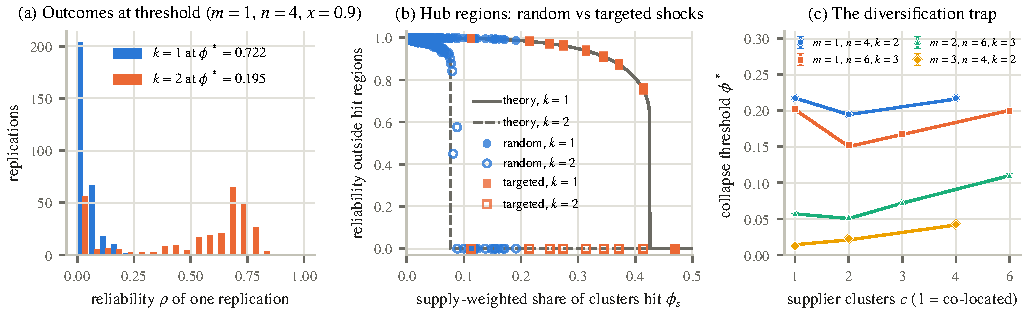
\includegraphics[width=\linewidth]{figures/fig_bimodal_hubs.pdf}
\caption{(a) Outcomes of 300 replications per configuration at the theoretical threshold: $k=1$ fades continuously, while $k=2$ is bimodal. (b) Supply concentrated in hub regions ($m=2$, $n=4$, $c=4$, $x=0.9$). Each point is one run, and the $y$-axis is reliability among firms whose own region was not hit. Random and targeted shocks both fall on the theory curve once the shock is measured by the supply-weighted share of hit clusters.}
\label{fig:hubs}
\end{figure}

\paragraph{Realism variants (H4).} We tested two departures from the homogeneous model. First, we gave suppliers heavy-tailed popularity, choosing them within a region with probability proportional to a Pareto fitness of shape 2.0 or 1.25 (CNST's degree tails). This changed mean reliability by at most 0.002 for $k=1$, and for $k=2$ by at most 0.03, at the threshold where the run-to-run spread is 0.35, so within noise. The theory is robust to hub suppliers, since a hub's functionality does not depend on its popularity. Second, we concentrated \emph{supply} geographically: supplier clusters choose region $g$ with probability proportional to a Pareto(1.25) weight, while firms stay spread evenly, so the largest region hosts 11\% of all supply relationships but only 0.5\% of firms. We then hit either the $h$ largest-supply regions (targeted) or $h$ random ones. Hitting the single largest region, only 0.5\% of firms, collapses the $k=2$ network completely, while hitting up to 10 random regions (5\% of firms) collapses it in only 5\% of runs, namely those whose draw happens to include a large-supply region. As shown in Figure~\ref{fig:hubs}(b), every run falls on the theory curve once $\phi$ in Equation~\eqref{eq:model} is replaced by the supply-weighted share of hit clusters $\phi_s$ (mean absolute error 0.002). Therefore, the quantity that governs collapse is the share of supply relationships in the shocked area, not its share of firms or output.

\section{Discussion and Further Research}
CNST's disaster area held 4.6\% of output, inside the $\phi^*$ range of our $k=2$ networks, and our hub experiment shows that supply-weighted exposure can far exceed output share. The smooth propagation CNST observed therefore suggests that Japan's effective $k$ was low, its supplier geography favorable, or its $x$ well above $\xc$. This is a hypothesis, since output share and region share differ, but it is testable: re-estimate CNST's design using the share of each firm's suppliers in the disaster area instead of minimum distance, look for a kink where fewer than $k$ suppliers survive, and test for bimodal outcomes and exit spikes among the most exposed firms. On the theory side, the next steps are proving the geography conjecture, making $c$ endogenous to test whether firms under-diversify geographically (EGL's reliability externality suggests they will), and moving to configuration-model graphs with cycles. Choosing which firms to harden under a budget is a reverse influence-maximization problem \cite{kempe2003}, but the AND across inputs likely breaks submodularity, leaving greedy guarantees open.

\section{Conclusion}
Our model shows that redundancy requirements and correlated shocks together make supply networks more fragile than EGL's independent-shock model suggests. Moving from $k=1$ to $k=2$ cuts the tolerable regional shock from 42.5\% to 7.7\% of regions, co-location roughly halves it again, and even perfect spreading only converts a regional shock into EGL's systemic one. Simulations confirm the theory and the all-or-nothing collapse, and teach a practical lesson: measure exposure by a region's share of supply relationships, since hitting one region with 0.5\% of firms collapsed a $k=2$ network.

\newpage
\renewcommand{\refname}{References}
{\small
\begin{thebibliography}{99}\setlength{\itemsep}{1pt}
\bibitem{egl2022} M.~Elliott, B.~Golub, and M.~V.~Leduc. Supply network formation and fragility. \emph{American Economic Review}, 112(8):2701--2747, 2022.
\bibitem{cnst2021} V.~M.~Carvalho, M.~Nirei, Y.~U.~Saito, and A.~Tahbaz-Salehi. Supply chain disruptions: Evidence from the Great East Japan Earthquake. \emph{Quarterly Journal of Economics}, 136(2):1255--1321, 2021.
\bibitem{buldyrev2010} S.~V.~Buldyrev, R.~Parshani, G.~Paul, H.~E.~Stanley, and S.~Havlin. Catastrophic cascade of failures in interdependent networks. \emph{Nature}, 464:1025--1028, 2010.
\bibitem{centola2007} D.~Centola and M.~Macy. Complex contagions and the weakness of long ties. \emph{American Journal of Sociology}, 113(3):702--734, 2007.
\bibitem{dorogovtsev2006} S.~N.~Dorogovtsev, A.~V.~Goltsev, and J.~F.~F.~Mendes. $k$-core organization of complex networks. \emph{Physical Review Letters}, 96:040601, 2006.
\bibitem{ek2010} D.~Easley and J.~Kleinberg. \emph{Networks, Crowds, and Markets: Reasoning About a Highly Connected World}. Cambridge University Press, 2010.
\bibitem{granovetter1978} M.~Granovetter. Threshold models of collective behavior. \emph{American Journal of Sociology}, 83(6):1420--1443, 1978.
\bibitem{kempe2003} D.~Kempe, J.~Kleinberg, and \'E.~Tardos. Maximizing the spread of influence through a social network. In \emph{Proc.\ ACM SIGKDD}, pp.\ 137--146, 2003.
\bibitem{kleinberg2007} J.~Kleinberg. Cascading behavior in networks: Algorithmic and economic issues. In N.~Nisan et al., eds., \emph{Algorithmic Game Theory}. Cambridge University Press, 2007.
\end{thebibliography}
}

\paragraph{AI use acknowledgment.} We used Claude (Anthropic) to help condense our drafts, write the simulation code, and format this paper. We reviewed the analysis, reran the code, and checked every reported number against its output.
\end{document}
